\subsubsection{Building A Decentralised Platform}

The criteria established by the user design and the specific requirements and philosophies of the architecture yields the specific technology stack discussed below. This stack provides the backbone upon which the implementation presented is based.

\begin{figure}[H]
  \centering
  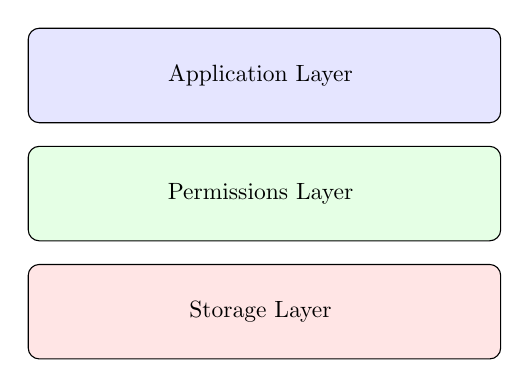
\begin{tikzpicture}[scale = 0.6, every node/.style={scale = 0.85}, every node/.append style={fill = white, rounded corners = 2pt, inner sep = 2pt, align = center}]
  
  % Layer boxes
  \draw [rounded corners, fill=blue!10] (-5, 3.5) rectangle (5, 1.5);
  \node [fill=blue!10] at (0, 2.5) { Application Layer };
  
  \draw [rounded corners, fill=green!10] (-5, 1) rectangle (5, -1);
  \node [fill=green!10] at (0, 0) { Permissions Layer };
  
  \draw [rounded corners, fill=red!10] (-5, -3.5) rectangle (5, -1.5);
  \node [fill=red!10] at (0, -2.5) { Storage Layer };
  
  \end{tikzpicture} \\
  \caption{
  	Platform Layers Overview
  }{
  	An overview of the layers of the platform from top to bottom. The permissions layer conceptually lies between the application layer and the storage layer, although in a decentralised system these layers act independently.
  }
  \label{fig:archi_platform_layers}
\end{figure}

The above layers shown in figure \ref{fig:archi_platform_layers} are discussed below in order of design importance, i.e. the permissions layers is at the centre of the application and somewhat defines the design of the other two layers.

\paragraph{Permissions Layer}

As per the architecture criteria, the correct blockchain technology to use for this project is one compatible with an already developed and established public network. The four considered networks were \href{https://bitcoin.org/en/}{Bitcoin Blockchain}, \href{https://www.ethereum.org/}{Ethereum} (Ether), \href{https://www.hyperledger.org/}{Hyperledger}, and \href{https://www.corda.net/}{R3 Corda}. Whilst the blockchain technology being used for the project remains as only a proof of concept, the exact technology and it's shortcomings are not completely relevant. For this project, the exact cost of transacting with a particular chain will not be considered, with the ease of use, ability to integrate, and security proving to be the priority.

Bitcoin Blockchain, whilst the first widespread use of a public decentralised ledger, is designed as a cryptocurrency network foremost. This means there are strict limitations on the size of data that is contained by a transaction and the scripting language used has requirements to guarantee security during transfer of funds. It is not a blockchain designed with an application layer that is accessible to developers. This does not mean it is not possible to create applications on the Bitcoin Blockchain, but there are more suitable alternatives we can consider.

R3 Corda and Hyperledger both offer approaches engineered towards the demands of business and sharing application data globally. They both state they restrict the viewing of transactions to only those whom the transaction concerns. They both also have development environments available to allow building applications on their respective networks. 

With this said, Ethereum remains the standout choice for an application of this nature. Whilst Ethereum maintains the global transaction history as per the Bitcoin Blockchain, the development environment and ease of creating an application layer built atop the service provided a solution that most closely met the criteria of this project at this stage. The availability of \href{https://github.com/trufflesuite/truffle}{Truffle}~\footnote{As a pre-cursor to this project I fixed issues with a current boilerplate using Truffle and created my own boilerplate \href{https://github.com/FreddieLindsey/truffle-webpack-boilerplate}{repository}, available to the public to aid in future DApp creation.} (amongst other Ethereum development frameworks) and \href{https://github.com/ethereum/solidity}{Solidity} make creating contracts and deploying them relatively easy. Furthermore the availability of a local testnet~\footnote{EthereumJS offers \href{https://github.com/ethereumjs/testrpc}{testrpc} a JavaScript implementation of an Ethereum node which allows fast and extensible private, local node setup.} makes developing contracts in a secure environment possible.

\paragraph{Storage Layer}

Distributed (but centralised) storage, of the likes of Amazon Web Services S3 etc., is not suitable for this application. Whilst highly performant, a single corporation maintains the right to terminate the service at any juncture. This is not compatible with the objectives of this project.

Storj was considered as above, however this project is not intending to use a currently implemented system for private data sharing, but provide it's own solution to the data sharing problem. Therefore, Storj will not be used.

Whilst still in its infancy, a JavaScript implementation of an IPFS client \href{https://github.com/ipfs/js-ipfs}{is available} and has basic functionality allowing the putting and getting of objects onto and from the IPFS network.

\paragraph{Application Layer}

As part of this project's intentions to create a proof of concept demonstration, a reference implementation of a client interface is necessary. This interface should be completely visual, require no special knowledge from any user, and be intuitive and as simple as possible. It should be as accessible as possible with current technology, allowing any prospective user to experiment with the capabilities of the platform.

Staying in the vein of a completely decentralised platform, it would be the intention that the application is deployed to a form of decentralised storage (as discussed above) and that it once again requires no third party or centralised endpoint.

For these reasons, the reference interface will be created using client-side routing, built entirely in browser-compatible JavaScript, and usable on any web browser. This will allow the user to navigate as they usually would on any other web-based application, but without the need to make any further requests~\footnote{The user will need to make an initial request to download the application and load it into the browser. Assuming that the application is cached locally using a local storage node, the time to load the application will be negligible.}. The only user-trigger requests that will be made will be to the permissions and storage layers of the platform, which are themselves decentralised.

% TODO: Maybe talk about Webpack / React / ES6
